\scanpage{47}
\unsure{Le schéma suivant associé à} $G$ \unsure{est exact} de \unsure{groupes} sur $S$
\diagram{\begin{tikzcd}[ampersand replacement=\&]
e \arrow[r] \& \unsure{H_1^\rho} \arrow[r] \& \Gamma_1^\rho \arrow[r,dash] \& E_1^\rho \arrow[r,dash] \& e
\end{tikzcd}}
\[
\Gamma_1^\rho\simeq E_1^\rho.\unsure{H_1^\rho}
\]
qui permet d'écrire
\diagram{\begin{tikzcd}[ampersand replacement=\&,column sep=large]
H^0(S,E_1^\rho) \arrow[r] \& H^1(S,\unsure{H_1^\rho}) \arrow[r] \& H^1(S,\Gamma_1^\rho) \arrow[r] \arrow[d,equal] \& H^1(S,E^\rho)\\
\&\& H^1(S,\Gamma)\&
\end{tikzcd}}

\deleted{\unsure{On sait}}
A priori, l'application envisagée n'est pas injective. \deleted{\unsure{Ainsi}}\inserted{\unsure{Cependant}} l'ens des éléments de $H^1(S,\unsure{H_1^\rho})$ qui donnent l'élément neutre de $H^1(S,\Gamma_1^\rho)$ \deleted{\unsure{est celui qui}} est en correspondance biunivoque avec $H^0(S,E^\rho)/\operatorname{Im}H^0(S,\Gamma^\rho)$, est trivial puisque $\Gamma_1^\rho$ est un produit \unsure{semi-direct}.

Mais si $\xi\in H^1(S,\unsure{H_1^\rho})$, on peut utiliser $\xi$ pour tordre encore la situation, on trouve
\diagram{\begin{tikzcd}[ampersand replacement=\&,column sep=small]
e \arrow[r] \& (\unsure{H_1^\rho})^\xi \arrow[r] \& (\Gamma_1^\rho)^\xi \arrow[r] \arrow[d,equal] \& (E_1^\rho)^{\deleted{\unsure{\xi}}} \arrow[r] \& e\\
e \arrow[r] \& \operatorname{Ad}(G) \arrow[r,dash] \& \operatorname{Aut}(G) \arrow[r,dash] \& \operatorname{Ext}(G) \arrow[r] \& e
\end{tikzcd}}
et ici on est ramené à la question si tout automorphisme ext. de $G$ provient d'un automorphisme. Ce n'est pas du tout évident quand $G$ n'est \deleted{\unsure{automorphisme}} pas une forme extérieure type. [i.e. \deleted{\unsure{un groupe}} n'\unsure{a} pas de ss-groupe de Borel $\supset$ Tore maximal].

\margin{\figure{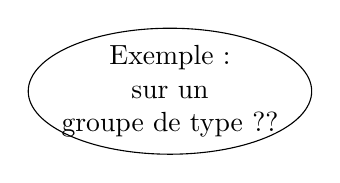
\begin{tikzpicture}\node[align=center] at (0,0) {\uline{Exemple} :\\\unsure{sur un}\\\unsure{groupe de type} ??};\draw (0,0) ellipse (1.8 and .8);\end{tikzpicture}}}
\margin{Faux sur $\mathbb R$ avec les formes \unsure{diverses} (\unsure{groupe unitaire}) : deux formes hermitiennes \unsure{opposées|voisines} donnant le \unsure{même} groupe algébrique sur $\mathbb R$ mais \uline{\unsure{ne sont pas}} isom.}
\margin{46}
